\section{Introduction}\label{sec:intro}

Variational Autoencoders (VAEs) \citep{kingma2014autoencoding, rezende2014stochastic} are latent variable models parameterized by deep neural networks and trained with variational inference. Recently, it has been shown that VAEs with hierarchical structures of latent variables \citep{ranganath2016hierarchical}, coupled with skip-connections \citep{maaloe2019biva, So_nderby2016-en}, can generate high-quality images \citep{Child2020-ze, vahdat2020nvae}. An interesting trait of VAEs is that they allow learning meaningful latent space that could be further used in downstream tasks \citep{bengio2013representation, higgins2017darla}. These successes of VAEs motivate us to explore the \textit{robustness} of the resulting latent representations to better understand the capabilities and potential vulnerabilities of VAEs. Here, we focus on \textit{adversarial attacks} on VAEs to verify robustness of latent representations that is especially important in such applications as anomaly detection \citep{an2015variational, maaloe2019biva} or data compression \citep{balle2018variational, habibian2019video}. 

The main questions about adversarial attacks for VAEs are mainly focused on how they could be formulated and alleviated. In \citet{Gondim-Ribeiro2018-cu}, it is proposed to minimize the KL-divergence between an adversarial input and a target input to learn an adversarial attack for the vanilla VAE. Further, in \citet{kuzina2021adv}, it is shown that a similar strategy can be used to attack hierarchical VAEs. To counteract the adversarial attacks, \citet{Willetts2019-mu} suggest using a modified VAE objective, namely, $\beta$-TCVAE, that increases VAE robustness, especially when coupled with a hierarchical structure. It was shown in \citet{camuto2021towards} that $\beta$-VAEs tend to be more robust to adversarial attacks in terms of the $r$-metric proposed therein. \citet{barrett2021certifiably} reported that the adversarial robustness can be achieved by constraining the Lipschitz constant of the encoder and the decoder. \citet{cemgil2020autoencoding, Cemgil2019-vn} introduced modifications in the VAE framework that allow for better robustness against the adversarial attacks on downstream classification tasks. In our work, we consider $\beta$-VAE, $\beta$-TCVAE and a hierarchical VAE, and outline a defence strategy that improves robustness to attacks on the encoder and the downstream classification task. The proposed method is applied during inference and, therefore, can be combined with other known techniques to get more robust latent representations.


An adversarial attack on a VAE is usually formulated as an additive perturbation $\varepsilon$ of the real data point $\rvx^r$ so that the resulting point is perceived by a model as if it is a totally different image (either during reconstruction or in the downstream classification task) \citep{Gondim-Ribeiro2018-cu}. In Figure~\ref{fig:toy_exaple}, we depict an example of an attack on the encoder. The reference point $\rvx^r$ and the adversarial point $\rvx^a$ are almost indistinguishable, but they are encoded into different regions in the latent space. As a result, their reconstructions also differ significantly.

% \begin{wrapfigure}{r}{0.53\textwidth}
\begin{figure}[t]
	% \vskip -100pt
	\begin{center}
		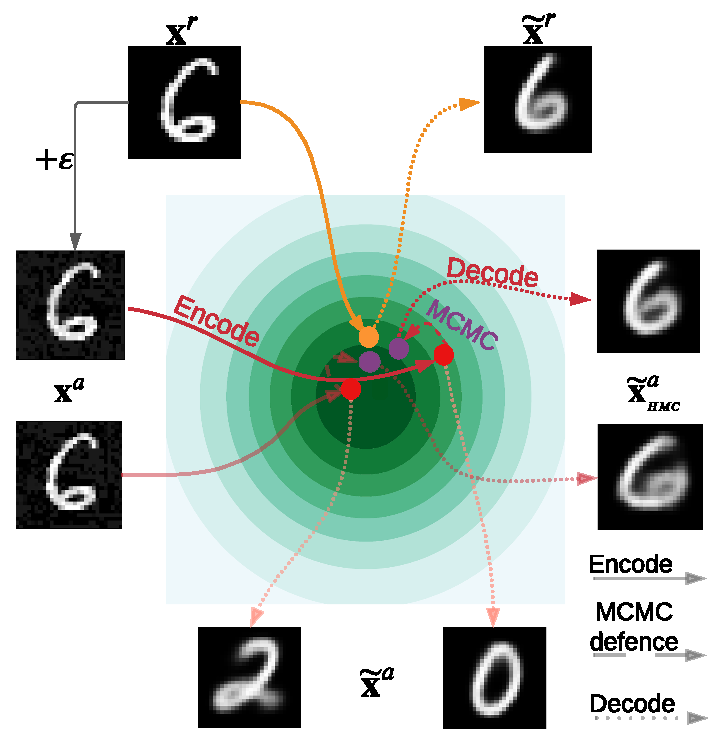
\includegraphics[width=0.6\linewidth]{pics/3_adv_att/Figure_1_upd.pdf}
		\caption{An example of an unsupervised encoder attack on VAE with 2D latent space and the proposed defense. 
			Given a single reference point $\rvx^r$ we learn additive perturbation $\varepsilon$, s.t. perturbed input $\rvx^a$ has the most different latent code and therefore the reconstruction $\widetilde{\rvx}^a$. 
			We observe that a single reference point can be mapped to extremely different regions of the latent space but using MCMC we are able to move them closer to the initial position so that the reconstruction $\widetilde{\rvx}^a_{\text{\tiny{HMC}}}$ is similar to the initial one $\widetilde{\rvx}^r$.}
		\label{fig:toy_exaple}
	\end{center}
    \vspace{\baselineskip}
\end{figure}
% \end{wrapfigure}

In this paper, we propose the method motivated by the following hypothesis: \textit{An adversarial attack maps the input to a latent region with a lower probability mass assigned by the true posterior (proportional to the conditional likelihood times the marginal over latents) and, eventually, we obtain incorrect reconstructions}. 
Therefore, a potential manner to alleviate the effect of an attack may rely on running a Markov chain to move the latent representation back to a more probable latent region. 
Such a defence is reasonable because we do not modify the training procedure or the model itself, we only insert a correction procedure. As a result, we propose to counteract adversarial attacks by enhancing the variational inference with Markov Chain Monte Carlo (MCMC) sampling. 
The illustrative example depicted in the Figure \ref{fig:toy_exaple} shows that the latent code of the adversarial input (red circle) moves closer to the latent code of the reference point (orange circle) after applying the MCMC (purple circle). 


The contribution of this work is the following:
\begin{itemize}%[leftmargin=*]
    \item We propose to use an MCMC technique during inference to correct adversarial attacks on VAEs.
    \item We show theoretically that the application of an MCMC technique could indeed help to counteract adversarial attacks (Theorem \ref{theorem:main}).
    \item We indicate empirically that the previously proposed strategies to counteract adversarial attacks do not generalize well across various datasets.
    \item We show empirically that the proposed approach (i.e., a VAE with an MCMC during inference) outperforms all baselines by a significant margin.
\end{itemize}

% In Figure \ref{fig:toy_exaple} we show an example of the \textit{supervised} attack on VAE with the 2D latent space. We show that we can add noise $\epsilon$ to a reference image so that the resulting adversarial input (second column) is encoded to a new point in the latent space. This new point is defined by the target image (first column). In \textit{unsupervised} attacks, on the other hand, we assume that the target image is not given. We show that it is still possible to construct an effective attack in this setting. The research goals of this work are the following:
% \begin{itemize}[leftmargin=*]
%     \item Defining robustness measures to understand how VAEs behave for adversarial attacks both in the latent space and the pixel space.
%     \item Assessing robustness of hierarchical and $\beta$-VAEs to adversarial attacks.
%     \item \jt{We need to add a bullet about MCMC to the rescue!}
% \end{itemize}